\documentclass[compress,handout,10pt]{beamer}

\newlength{\wideitemsep}
\setlength{\wideitemsep}{\itemsep}
\addtolength{\wideitemsep}{100pt}
\let\olditem\item
\renewcommand{\item}{\setlength{\itemsep}{0.5\baselineskip}\olditem}

\usetheme{Singapore}
\usecolortheme{lily}
\usefonttheme[onlymath]{serif}

\usepackage{float}
\floatstyle{boxed}
\usepackage{colortbl}
\usepackage{mathpazo}
\usepackage{graphicx}
\usepackage{movie15}
\usepackage{bm}
\usepackage{verbatim}
\usepackage{comment}
\usepackage{caption}
\usepackage{subcaption}
\captionsetup[subfigure]{labelformat=empty}
\captionsetup[figure]{labelformat=empty}

\newcommand{\mygreen}{\color{green!50!black}}
\newcommand{\myblue}{\color{blue}}
\newcommand{\myred}{\color{red}}
\newcommand{\mycolor}{\color{red}{c}\color{blue}{o}\color{green}{l}\color{orange}{o}\color{cyan}{r}}
\newcommand{\mysize}{\scriptsize{s}\small{i}\normalsize{z}\Large{e}}
\newcommand{\myshape}{\textcircled{s}\textit{h}\texttt{a}\textsf{p}\textsc{e}}

\xdefinecolor{titlecolor}{rgb}{.855,.647,.125}
\setbeamercolor{frametitle}{fg=titlecolor}
\setbeamerfont{frametitle}{series=\bfseries}
\setbeamercolor{normal text in math text}{parent=math text}

\setbeamertemplate{navigation symbols}{} %gets rid of navigation symbols
\setbeamertemplate{footline}[frame number]
\beamertemplateshadingbackground{blue!5}{yellow!10}


\graphicspath{{./images/}{}}

\title{{\color{blue} \LARGE 550.400: Mathematical Modeling and Consulting\newline} }

\subtitle{{\color{red} \large Lecture Notes} }

\author{ 
%    \vspace{5pt}
    {\bf{Instructor:}} \\ 
Dr.~N.~H.~Lee \\ 
    \vspace{5pt}
} 
\institute{JHU AMS 2013 Spring}

\date{\mygreen Last Complied on \today} 

\begin{document}

\begin{frame}[plain]
    \titlepage
\end{frame}

\begin{frame}
    \frametitle{Outline}
    \tableofcontents
\end{frame}

\section{Guessing Ages}
\begin{frame}
    \frametitle{How to Play}
    \vspace{7pt}
    \begin{figure}
        \begin{center}
            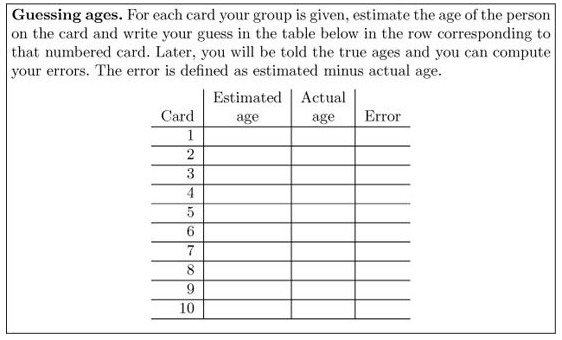
\includegraphics[width=\textwidth]{images/guessingagesrule.png}
        \end{center}
    \end{figure}
\end{frame}

\begin{frame}
    \frametitle{Example}
    \vspace{7pt}
    \begin{figure}
        \begin{center}
            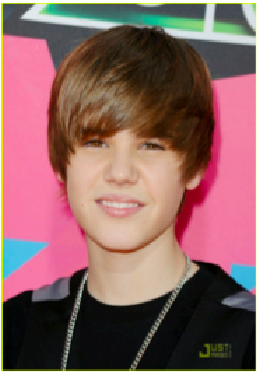
\includegraphics[height=0.8\textheight]{images/JustinBieber.png}
        \end{center}
    \end{figure}
\end{frame}

\begin{frame}
    \frametitle{Sample output}
    \vspace{7pt}
    \begin{figure}
        \begin{center}
            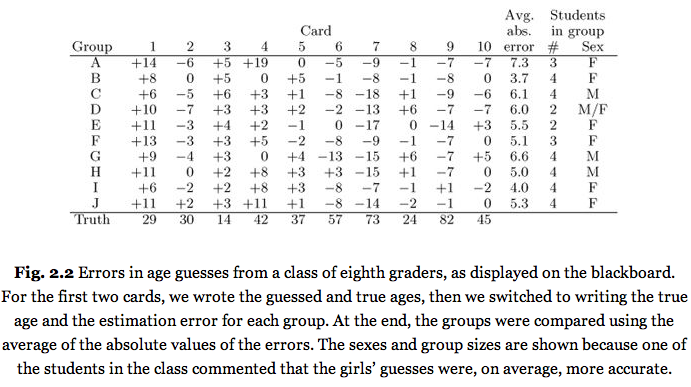
\includegraphics[width=\textwidth]{images/guessing-ages-error.png}
        \end{center}
    \end{figure}
\end{frame}

\section{Where are the cancers?}

\begin{frame}
    \frametitle{What do you notice?}
    \vspace{7pt}
    \begin{figure}
        \begin{center}
            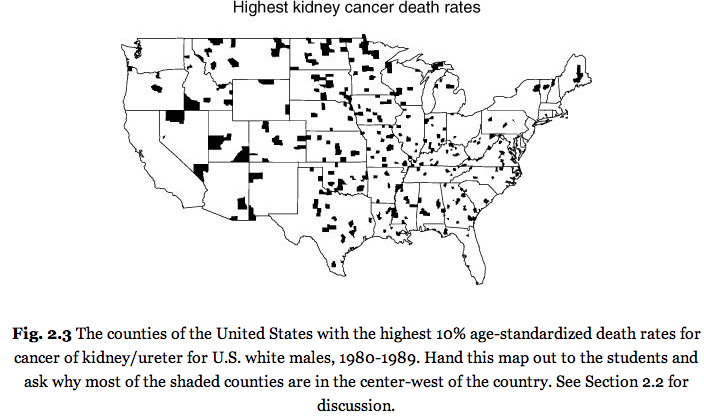
\includegraphics[width=\textwidth]{images/HighestKidneyCancerDeathRate.png}
        \end{center}
    \end{figure}
\end{frame}

\begin{frame}
    \frametitle{What do you notice?}
    \vspace{7pt}
    \begin{figure}
        \begin{center}
            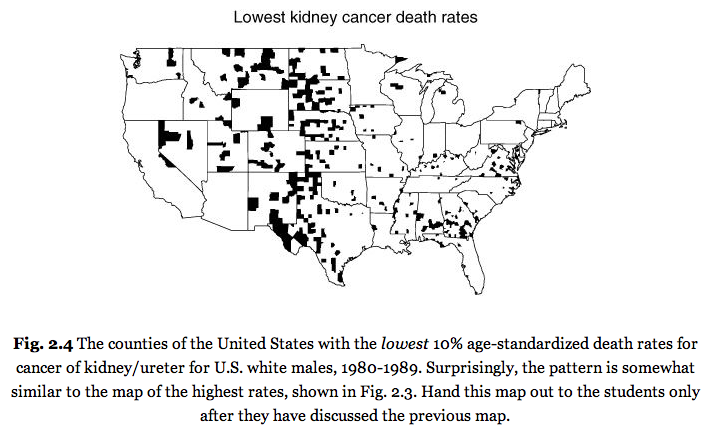
\includegraphics[width=\textwidth]{images/LowestKidneyCancerDeathRate.png}
        \end{center}
    \end{figure}
\end{frame}

\section{Handedness inventory}
\begin{frame}
    \frametitle{Are you left-handed or right-handed?}
    \vspace{7pt}
    \begin{figure}
        \begin{center}
            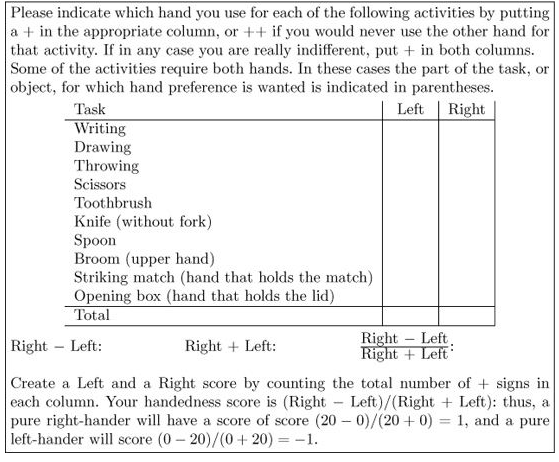
\includegraphics[width=0.9\textwidth]{images/HandednessInventory.png}
        \end{center}
    \end{figure}
\end{frame}

\section{What's in the news?}
\begin{frame}
    \frametitle{The first topic}
    \begin{figure}
    \caption{\emph{New York Times}, March 1, 1995} 
        \centering    
        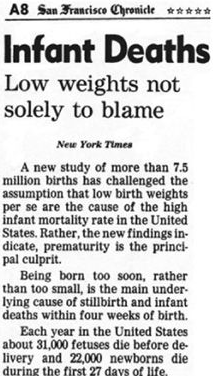
\includegraphics[width=0.37\textwidth]{images/OnInfantDeathPart1.png}
        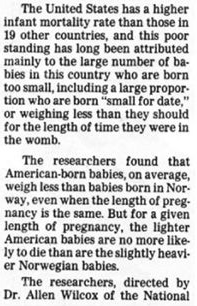
\includegraphics[width=0.37\textwidth]{images/OnInfantDeathPart2.png}
    \end{figure}
\end{frame}

\end{document}
